\documentclass{standalone}
\usepackage{tikz}
\usetikzlibrary{decorations.pathreplacing}
\usepackage{amsfonts}

\begin{document}
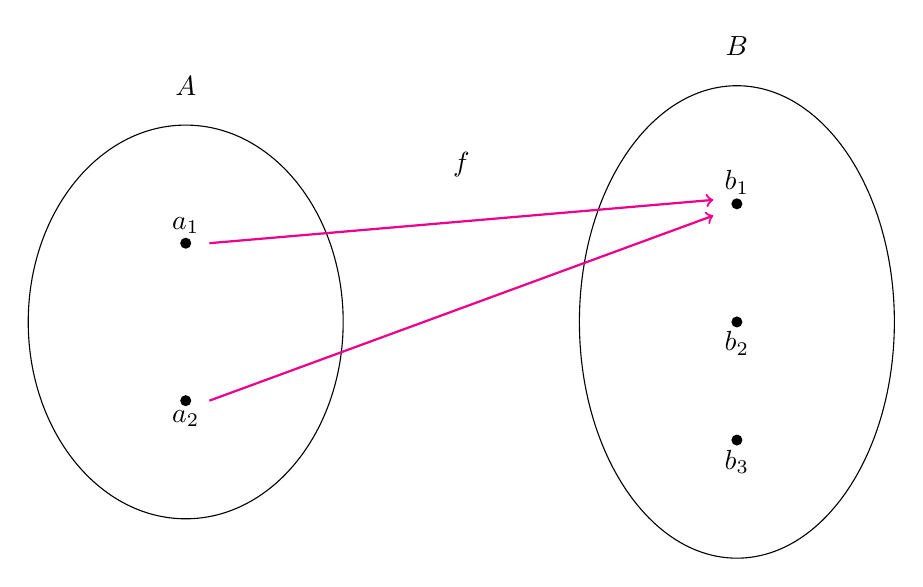
\begin{tikzpicture}
  % Ellipse A
  \draw (0,0) ellipse (2cm and 2.5cm);
  \node at (0, 3) {$A$};
  \fill (0, 1) circle (2pt) node[above] {$a_1$};
  \fill (0, -1) circle (2pt) node[below] {$a_2$};
  
  % Ellipse B
  \draw (7,0) ellipse (2cm and 3cm);
  \node at (7, 3.5) {$B$};
  \fill (7, 1.5) circle (2pt) node[above] {$b_1$};
  \fill (7, 0) circle (2pt) node[below] {$b_2$};
  \fill (7, -1.5) circle (2pt) node[below] {$b_3$};
 
   % Arrow from a_1 to b_1
  \draw[->][magenta, thick] (0.3, 1) -- (6.7, 1.55);
  
   % Arrow from a_2 to b_1
  \draw[->][magenta, thick] (0.3, -1cm) -- (6.7cm, 1.35cm);
  
    % Label "f" on top of the arrow
  \node at (3.5cm, 2cm) {$f$};
   
    \end{tikzpicture}
\end{document}